% The Generous Auction — explainer. Compile with: xelatex generous-auction.tex (twice)
% TeX Live basic: uses only fontspec, geometry, xcolor, amsmath, unicode-math, booktabs,
% tikz, hyperref, microtype. No pgfplots, no tcolorbox.
\documentclass[11pt]{article}

\usepackage{fontspec}
\usepackage[margin=2.4cm,top=2.2cm,bottom=2.4cm]{geometry}
\usepackage{xcolor}
\usepackage{amsmath}
\usepackage{unicode-math}
\usepackage{booktabs}
\usepackage{tikz}
\usepackage{microtype}
\usepackage[colorlinks=true,linkcolor=accent,urlcolor=accent,citecolor=accent]{hyperref}

\definecolor{accent}{HTML}{1F5C99}
\definecolor{ink}{HTML}{1A1A1A}
\definecolor{soft}{HTML}{6E6A63}
\definecolor{rulec}{HTML}{D8D4CC}
\definecolor{boxbg}{HTML}{F4F2EE}
\definecolor{cT3}{HTML}{8E5BA6}
\definecolor{cT2}{HTML}{2F7DBF}
\definecolor{cT1}{HTML}{D9822B}
\definecolor{cT0}{HTML}{3E9E6E}
\definecolor{dead}{HTML}{B8B3AA}

\setmainfont{Charter}[Numbers=OldStyle]
\setmonofont{Menlo}[Scale=0.82]
\setsansfont{Helvetica Neue}
\setmathfont{latinmodern-math.otf}   % by filename: not registered under a family name here

\color{ink}
\hypersetup{pdftitle={The Generous Auction},pdfauthor={},pdfsubject={Geometric pay-as-bid tick book}}

% --- headings (titlesec is not in TeX Live basic; redefine by hand) --------
\makeatletter
\renewcommand\section{\@startsection{section}{1}{\z@}%
  {1.5em \@plus .3em \@minus .2em}{0.5em}%
  {\sffamily\large\bfseries\color{accent}}}
\renewcommand\subsection{\@startsection{subsection}{2}{\z@}%
  {1.1em \@plus .2em \@minus .1em}{0.35em}%
  {\sffamily\normalsize\bfseries\color{ink}}}
\renewcommand\paragraph{\@startsection{paragraph}{4}{\z@}%
  {0.9em \@plus .2em \@minus .1em}{-0.6em}%
  {\sffamily\bfseries\color{ink}}}
\makeatother

% --- a lightweight callout box (no tcolorbox in TeX Live basic) ------------
\newcommand{\callout}[1]{%
  \par\medskip\noindent
  \begin{tikzpicture}
    \node[fill=boxbg,inner sep=9pt,text width=\dimexpr\linewidth-24pt\relax,align=justify] (b) {#1};
    \draw[accent,line width=2.2pt] (b.north west) -- (b.south west);
  \end{tikzpicture}\par\medskip}

\newcommand{\tick}[1]{\textcolor{#1}{\rule[0.15ex]{1.6ex}{1.6ex}}}
% Neither Charter nor LM Math carries U+2713; draw it instead of shipping a tofu box.
\newcommand{\ok}{\tikz[baseline=-0.15ex,scale=0.115]
  \draw[cT0,line width=1.3pt,line cap=round,line join=round] (0,1.1)--(0.95,0)--(2.5,2.4);}
\renewcommand{\arraystretch}{1.15}

\begin{document}

% ==========================================================================
\begin{center}
{\sffamily\Huge\bfseries\color{accent} The Generous Auction}\\[0.45em]
{\sffamily\large\color{soft} A geometric pay-as-bid tick book, worked through by hand}\\[0.9em]
{\color{soft}\rule{0.32\linewidth}{0.6pt}}
\end{center}
\vspace{0.4em}

\noindent
This note explains the distribution rule proposed for the MONO auction: how one round's
emission is split across the order book, why the split has the shape it does, and how the
whole thing collapses into a single number that a contract can read in constant time. Every
number in the worked examples was recomputed from scratch rather than copied from the spec.

\callout{\textbf{Status.} The rule below is implemented twice: \texttt{src/GenerousAuction.sol}
for a single sale, and \texttt{src/MonoAuction.sol} for the same mechanism behind a
multi-market wrapper. Both solve each round in one sweep over a bounded price window instead of
carrying the lazy accumulator of \S\ref{sec:acc}. \S\ref{sec:v1} describes the strict-priority
rule they replaced; \texttt{index.html} is an interactive model of both.}

% ==========================================================================
\section{The book}

The auction sells a fixed emission of tokens per round in exchange for a currency. Bids are
placed on a ladder of discrete price levels called \emph{ticks}. Tick $i$ carries a price
$p_i$, and the ladder is geometric in price:
\[
  p_i \;=\; \mathrm{floor}\cdot(1+\delta)^i .
\]

A bidder does not name a quantity. They escrow a \emph{budget} $b_i$ of currency at a tick,
and that budget stands there, round after round, until it is spent or withdrawn. The tick's
budget is the sum of everyone standing on it.

Two properties are fixed. Both predate this design and neither is touched by it:

\begin{itemize}\setlength\itemsep{2pt}
\item \textbf{Pay-as-bid.} You buy at \emph{your own} tick's price, not at a common clearing
      price. Sales are final.
\item \textbf{Pro-rata within a tick.} Whatever a tick spends in a round is divided among the
      bids standing on it in proportion to their budgets.
\end{itemize}

Everything that follows concerns exactly one question: \emph{how is a round's emission $R$
divided \textbf{between} ticks?}

% --------------------------------------------------------------------------
\subsection{The current answer, and its problem}
\label{sec:v1}

Today the rule is strict priority. Fill the highest tick completely, then the next, then the
next, until $R$ runs out. Whichever tick the emission happens to stop inside is the
\emph{marginal} tick; it fills partially, and everything below it gets nothing.

That is simple, and it is what every clearing auction does. It also produces a cliff. A bidder
one tick above the margin fills completely; a bidder one tick below gets nothing, this round
and possibly for many more. The outcome turns entirely on which side of the line you land on,
and the line moves with demand you cannot see.

The generous auction replaces that cliff with a gradient.

% ==========================================================================
\section{The rule}

Let $A$ be the set of \emph{live} ticks — those with budget remaining — and let
\[
  \tau \;=\; \max A
\]
be the highest live tick, the top of the book. Give every live tick a weight that decays
geometrically with its distance below the top:
\[
  \boxed{\;w_i \;=\; q^{\,\tau-i}\;}\qquad q\in(0,1].
\]

The top tick weighs $1$. Each step down multiplies by $q$. Normalising by
$W=\sum_{j\in A}w_j$, tick $i$ takes a share
\[
  s_i \;=\; \frac{w_i}{W}
\]
of the round's emission: $a_i = R\,s_i$ tokens, costing $c_i = a_i\,p_i$ of its budget.

So every live tick buys every round. Not equally — a tick four levels down at $q=0.5$ buys at
one-sixteenth the rate of the top — but continuously, with no threshold anywhere.

\begin{figure}[h]
\centering
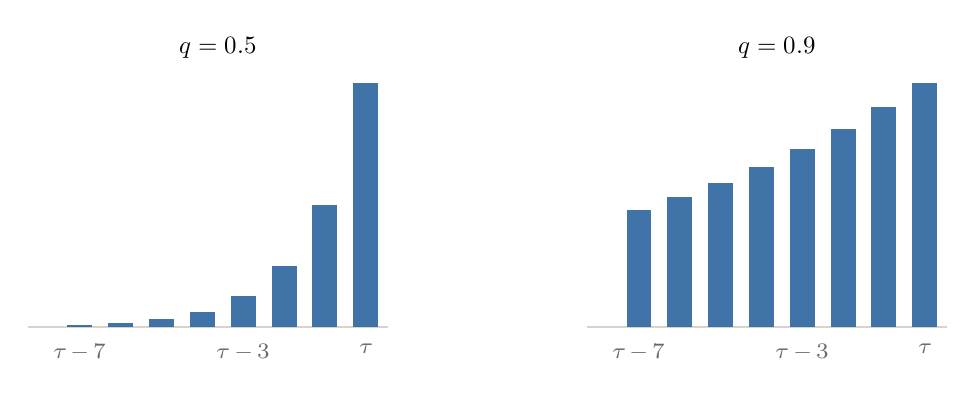
\begin{tikzpicture}[x=0.72cm,y=3.1cm]
  \foreach \panel/\qq/\lbl/\xoff in {0/0.5/{$q=0.5$}/0, 1/0.9/{$q=0.9$}/7.1}{
    \begin{scope}[xshift=\xoff cm]
      \draw[rulec,line width=0.5pt] (-0.45,0) -- (5.9,0);
      \foreach \d in {0,1,2,3,4,5,6,7}{
        \pgfmathsetmacro\h{pow(\qq,\d)}
        \pgfmathsetmacro\xx{5.5-\d*0.72}
        \fill[accent,opacity=0.85] (\xx-0.22,0) rectangle (\xx+0.22,\h);
      }
      \node[soft,font=\footnotesize\sffamily,anchor=north] at (5.5,-0.03) {$\tau$};
      \node[soft,font=\footnotesize\sffamily,anchor=north] at (5.5-3*0.72,-0.03) {$\tau-3$};
      \node[soft,font=\footnotesize\sffamily,anchor=north] at (5.5-7*0.72,-0.03) {$\tau-7$};
      \node[font=\small\sffamily,anchor=south] at (2.9,1.06) {\lbl};
    \end{scope}}
\end{tikzpicture}
\caption{The weight ladder $w=q^{\tau-i}$. Small $q$ concentrates the emission at the top of
the book; large $q$ spreads it far down. The knob is continuous.}
\end{figure}

% --------------------------------------------------------------------------
\subsection{The waterfall}

A tick's budget is finite, so a tick can run out \emph{in the middle} of a round's emission.
When it does, it leaves $A$, and the remainder of that same emission is redistributed by
recomputed weights among the survivors. If a second tick exhausts, redistribute again. There
are at most as many redistributions as there are exhausted ticks.

This is how unfilled emission moves upward, and it is not a separate mechanism. It is what
renormalisation does on its own: when a tick leaves, $W$ shrinks, so every surviving share
$w_i/W$ grows — most of all at the top, which carries the most weight. Nothing is transferred
from the exhausted tick. The shares simply rescale.

If every tick exhausts, the leftover is recorded as \texttt{unsold}. Under the strict setting
this holds even when a single bidder is alone in the book: they still receive only their own
share, which is the round-level guarantee against a whale simply buying the emission.

% ==========================================================================
\section{Worked example: four rounds, one exhaustion}
\label{sec:ex1}

Take $\mathrm{floor}=1$, $\delta=5\%$, and three live ticks. Let $q=0.5$ and $R=70$ tokens
per round.

\begin{center}
\begin{tabular}{lrrrrr}
\toprule
& price $p_i$ & budget $b_i$ & weight $w_i$ & share $s_i$ & tokens/round \\
\midrule
\tick{cT2}~tick 2 \ ($\tau$) & 1.1025 & 100 & $1$      & $4/7 = 57.1\%$ & 40 \\
\tick{cT1}~tick 1            & 1.0500 & 210 & $0.5$    & $2/7 = 28.6\%$ & 20 \\
\tick{cT0}~tick 0            & 1.0000 & 500 & $0.25$   & $1/7 = 14.3\%$ & 10 \\
\midrule
\multicolumn{3}{r}{$W = 1.75$} & & & $R = 70$ \\
\bottomrule
\end{tabular}
\end{center}

\paragraph{Rounds 1--2.} Nothing exhausts, so the split is constant and both rounds are
identical. Per round, tick 2 takes $40$ tokens for $44.10$ of currency, tick 1 takes $20$ for
$21.00$, and tick 0 takes $10$ for $10.00$ --- so \emph{over the two rounds together} tick 2
has taken $80$ tokens for $88.20$, leaving it $11.80$; tick 1 has taken $40$ for $42.00$ and
tick 0 $20$ for $20.00$.

\begin{center}
\begin{tabular}{lrrrrr}
\toprule
& share & tokens/rd & currency/rd & budget after R1 & after R2 \\
\midrule
\tick{cT2}~tick 2 \ ($\tau$) & $4/7$ & 40 & 44.10 &  55.90 &  11.80 \\
\tick{cT1}~tick 1            & $2/7$ & 20 & 21.00 & 189.00 & 168.00 \\
\tick{cT0}~tick 0            & $1/7$ & 10 & 10.00 & 490.00 & 480.00 \\
\midrule
$\Sigma$ & & 70 & 75.10 & & \\
\bottomrule
\end{tabular}
\end{center}

\noindent
Tick 2 is the one to watch: it burns $44.10$ a round against a budget of $100$, so it cannot
survive a third.

\paragraph{Round 3 — the interesting one.} Tick 2 has $11.80$ left, which buys
$11.80/1.1025 = 10.70$ tokens. At a $4/7$ share it reaches that after only
\[
  10.70 \times \tfrac{7}{4} \;=\; 18.73 \text{ tokens of the } 70 \qquad (26.8\% \text{ of the round}),
\]
at which point its budget is gone. On that first slice tick 1 receives $5.35$ and tick 0
receives $2.68$.

Now tick 2 is out. The top becomes $\tau=1$, weights rebuild as $w_1=1,\ w_0=0.5$, so
$W=1.5$ and the shares are $2/3$ and $1/3$. The remaining $51.27$ tokens pour by \emph{those}:
tick 1 takes $34.18$, tick 0 takes $17.09$.

Tick 1's share jumped from $28.6\%$ to $66.7\%$ the instant tick 2 exhausted — mid-round,
without any explicit transfer.

\begin{center}
\begin{tabular}{lrrrrrrr}
\toprule
& \multicolumn{2}{c}{stage 1 — $W=1.75$} & \multicolumn{2}{c}{stage 2 — $W=1.5$}
& \multicolumn{3}{c}{round 3} \\
\cmidrule(lr){2-3}\cmidrule(lr){4-5}\cmidrule(lr){6-8}
& share & tokens & share & tokens & tokens & currency & budget left \\
\midrule
\tick{cT2}~tick 2 & $4/7$ & 10.70 & \multicolumn{2}{c}{\color{soft}exhausted}
                  & 10.70 & 11.80 & \phantom{00}0.00 \\
\tick{cT1}~tick 1 & $2/7$ & \phantom{0}5.35 & $2/3$ & 34.18 & 39.53 & 41.51 & 126.49 \\
\tick{cT0}~tick 0 & $1/7$ & \phantom{0}2.68 & $1/3$ & 17.09 & 19.77 & 19.77 & 460.23 \\
\midrule
$\Sigma$ & & 18.73 & & 51.27 & 70.00 & 73.08 & \\
\bottomrule
\end{tabular}
\end{center}

\noindent
The two stages are one emission, not two: $18.73 + 51.27 = 70$. Only the shares changed
partway through.

\begin{figure}[h]
\centering
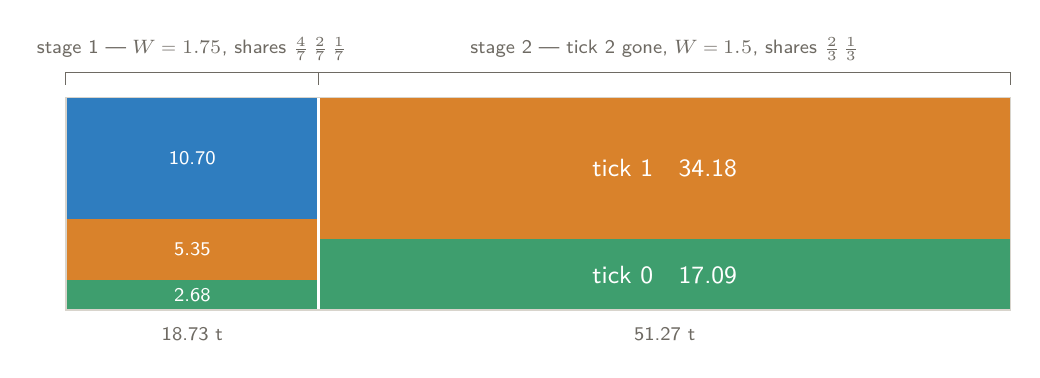
\begin{tikzpicture}[y=0.9cm]
  \def\Wd{12}
  % band 1: 18.73/70 of the width
  \def\bx{3.211}
  \fill[cT0] (0,0) rectangle (\bx,0.4286);
  \fill[cT1] (0,0.4286) rectangle (\bx,1.2857);
  \fill[cT2] (0,1.2857) rectangle (\bx,3);
  % band 2
  \fill[cT0] (\bx,0) rectangle (\Wd,1);
  \fill[cT1] (\bx,1) rectangle (\Wd,3);
  \draw[white,line width=1.1pt] (\bx,0) -- (\bx,3);
  \draw[rulec,line width=0.5pt] (0,0) rectangle (\Wd,3);
  % labels inside
  \node[white,font=\scriptsize\sffamily] at (\bx/2,2.15) {10.70};
  \node[white,font=\scriptsize\sffamily] at (\bx/2,0.86) {5.35};
  \node[white,font=\scriptsize\sffamily] at (\bx/2,0.21) {2.68};
  \node[white,font=\small\sffamily] at ({(\bx+\Wd)/2},2) {tick 1 \ \ 34.18};
  \node[white,font=\small\sffamily] at ({(\bx+\Wd)/2},0.5) {tick 0 \ \ 17.09};
  % brackets
  \draw[soft] (0,3.18) -- (0,3.35) -- (\bx,3.35) -- (\bx,3.18);
  \draw[soft] (\bx,3.18) -- (\bx,3.35) -- (\Wd,3.35) -- (\Wd,3.18);
  \node[soft,font=\scriptsize\sffamily,anchor=south] at (\bx/2,3.38)
    {stage 1 — $W=1.75$, shares $\tfrac47\,\tfrac27\,\tfrac17$};
  \node[soft,font=\scriptsize\sffamily,anchor=south] at ({(\bx+\Wd)/2},3.38)
    {stage 2 — tick 2 gone, $W=1.5$, shares $\tfrac23\,\tfrac13$};
  \node[soft,font=\scriptsize\sffamily,anchor=north] at (\bx/2,-0.1) {18.73 t};
  \node[soft,font=\scriptsize\sffamily,anchor=north] at ({(\bx+\Wd)/2},-0.1) {51.27 t};
\end{tikzpicture}
\caption{Round 3 of the example: the emission of 70 tokens, drawn left to right. Tick 2
(\tick{cT2}) exhausts 26.8\% of the way through; from that point the same round's remainder
flows by renormalised weights, and tick 1's rate more than doubles.}
\end{figure}

\paragraph{Round 4.} Two ticks left, shares $2/3$ and $1/3$: tick 1 takes $46.67$ tokens,
tick 0 takes $23.33$.

\begin{center}
\begin{tabular}{lrrrr}
\toprule
& share & tokens & currency & budget left \\
\midrule
\tick{dead}~tick 2 \ {\color{soft}(gone)} & — & — & — & \phantom{00}0.00 \\
\tick{cT1}~tick 1 \ ($\tau$) & $2/3$ & 46.67 & 49.00 & \phantom{0}77.49 \\
\tick{cT0}~tick 0            & $1/3$ & 23.33 & 23.33 & 436.90 \\
\midrule
$\Sigma$ & & 70.00 & 72.33 & \\
\bottomrule
\end{tabular}
\end{center}

\noindent
No renormalisation this round — the book did not change, so the shares from stage 2 of
round 3 simply carry over.

\paragraph{Totals over four rounds.}

\begin{center}
\begin{tabular}{lrrl}
\toprule
& currency spent & tokens bought & check \\
\midrule
\tick{cT2}~tick 2 & 100.00 \ (all of it) & 90.70  & $100/1.1025 = 90.70$ \\
\tick{cT1}~tick 1 & 132.51              & 126.20 & $77.49$ of budget still standing \\
\tick{cT0}~tick 0 & \phantom{0}63.10    & 63.10  & price is $1.0$ \\
\midrule
$\Sigma$ & 295.61 & \textbf{280.00} & $= 4R$ \ \ok \\
\bottomrule
\end{tabular}
\end{center}

Tick 1 and tick 0 are still standing with budget left, and they carry on into round 5 against
whoever bids next. Nothing was migrated, re-keyed, or refunded.

% ==========================================================================
\section{Why geometric}

The decay could have been any decreasing function of distance. Two properties single out
$q^{\,d}$, and both are load-bearing.

\subsection{Shift-invariance}

Because
\[
  \frac{q^{\,d+m}}{\sum_j q^{\,d_j+m}} \;=\; \frac{q^{\,d}}{\sum_j q^{\,d_j}},
\]
a new tick appearing \emph{above} the current top does not change the relative shares of
anyone already in the book. Everyone's weight is multiplied by the same $q^m$, which cancels.

This kills the obvious manipulation. Under a rule without this property, a nominal bid parked
far above the market stretches the curve and starves everyone below. Here it does nothing to
anyone else: the manipulator becomes the top tick and pays the top price for the privilege.
A hyperbolic weight $1/(1+d)$ does not have this property.

\subsection{Factorisability}

\[
  w_i \;=\; q^{\,\tau-i} \;=\; q^{\tau}\cdot q^{-i}
\]
splits into a purely global factor and a purely per-tick factor. This is what makes the whole
scheme computable lazily, and it is the subject of \S\ref{sec:acc}. With a hyperbolic weight
no such split exists, and reading a single bidder's position degrades to walking the entire
history of top-of-book changes.

\callout{One consequence to be clear about: distance is measured in \textbf{price ticks}, not
in rank among live ticks. A tick a hundred levels below the top receives $q^{100}\approx0$ even
if it happens to be the second-highest bid in the book. That is deliberate — the window of
participation is defined by distance in price, not by queue position. Rank would also destroy
laziness, since your rank changes when strangers bid.}

% ==========================================================================
\section{Worked example: exhaustion order is not price order}
\label{sec:ex2}

This example is short, and it is the one that dictates the data structure a contract needs.

The column that does the dictating is the last, the key $\kappa_i$. Track the draw with one scalar
$C$, the \emph{accumulator}, every live tick holding $q^{-i}\cdot C$ tokens. A tick takes its share
until its escrow is spent, then drops out --- at a fixed level of $C$, known before a token is
poured. That level is $\kappa_i$, so one sorted pass solves the whole waterfall.

Four live ticks one grid step apart, $q=0.5$, and a draw of $R=150$ tokens. Each tick holds escrow
$b_i$ (currency) at price $p_i$ (currency per token), so its \emph{capacity} in tokens is
$\mathrm{cap}_i = b_i/p_i$:

\begin{center}
\begin{tabular}{lrrrrrr}
\toprule
& escrow $b_i$ & price $p_i$ & capacity $\mathrm{cap}_i$ & $q^{-i}$ & opening share & key $\kappa_i$ \\
\midrule
\tick{cT3}~tick 3 \ ($\tau$) & \phantom{0}80 & 4 & \phantom{0}20  & 8 & $8/15 = 53.3\%$ & \phantom{00}2.5 \\
\tick{cT2}~tick 2            & 600           & 3 & 200            & 4 & $4/15 = 26.7\%$ & \phantom{0}50 \\
\tick{cT1}~tick 1            & \phantom{0}20 & 2 & \phantom{0}10  & 2 & $2/15 = 13.3\%$ & \phantom{00}5 \\
\tick{cT0}~tick 0            & 100           & 1 & 100            & 1 & $1/15 = \phantom{0}6.7\%$ & 100 \\
\midrule
\multicolumn{4}{r}{$V=\sum q^{-j} = 15$} & & & \\
\bottomrule
\end{tabular}
\end{center}

Column by column, with tick 3 as the worked instance:

\begin{itemize}\setlength\itemsep{1pt}
\item \textbf{escrow $b_i$} --- currency standing at the tick. An input.
\item \textbf{price $p_i$} --- currency per token there. An input; the four are one step apart.
\item \textbf{capacity $\mathrm{cap}_i = b_i/p_i$} --- most tokens that escrow can buy.
      Tick 3: $80/4 = 20$.
\item \textbf{weight $q^{-i}$} --- pull on each token poured; doubles per level up at $q=0.5$.
      Tick 3: $0.5^{-3} = 8$.
\item \textbf{opening share $q^{-i}/V$} --- weight over the live total $V=\sum_j q^{-j}=15$.
      Tick 3: $8/15 = 53.3\%$.
\item \textbf{key $\kappa_i = \mathrm{cap}_i\cdot q^{\,i}$} --- capacity per unit of weight, i.e.\
      $\mathrm{cap}_i/q^{-i}$: the level $C$ must reach for tick $i$ to exhaust.
      Tick 3: $20/8 = 2.5$.
\end{itemize}

\callout{Neither middle column is an allocation. \textbf{Capacity} is a ceiling: the most a tick
could ever take, if the draw were unlimited. \textbf{Opening share} is a rate: the fraction of
each marginal token a tick absorbs \emph{while every tick is still alive}. Tick 3's $53.3\%$
holds only for the first $37.5$ tokens, after which it is full and its share is redivided among
the survivors. The allocations themselves appear below, after the sweep.}

The key is $\kappa_i = \mathrm{cap}_i\cdot q^{\,i}$, and a tick exhausts exactly when the
accumulator reaches its key. Sorting by $\kappa$ gives the order in which ticks die:
\[
  \text{tick }3\ (2.5) \;\rightarrow\; \text{tick }1\ (5) \;\rightarrow\;
  \text{tick }2\ (50) \;\rightarrow\; \text{tick }0\ (100).
\]

\callout{\textbf{Tick 1 exhausts before tick 2, although tick 2 is priced higher and draws
twice the share.} Tick 1 is a small budget on a good level; tick 2 is a large budget one level
down. A rich low tick outlives a poor high tick. Exhaustion order and price order are
different orderings, and the contract must maintain the first one explicitly — the sorted
structure the current implementation gets for free from price is no longer sufficient.}

Running the draw, tracking a single scalar $C$ with $\Delta T = V\cdot\Delta C$:

\begin{center}
\begin{tabular}{clrrr}
\toprule
stage & event & tokens poured & $C$ after & $V$ after \\
\midrule
1 & tick 3 exhausts at $\kappa=2.5$   & \phantom{0}37.5 & \phantom{0}2.5 & 7 \\
2 & tick 1 exhausts at $\kappa=5$     & \phantom{0}17.5 & \phantom{0}5\phantom{.0} & 5 \\
3 & emission runs out first           & \phantom{0}95\phantom{.0} & 24\phantom{.0} & 5 \\
\bottomrule
\end{tabular}
\end{center}

Final allocation: tick 3 takes $20$ (its whole capacity), tick 1 takes $10$ (likewise),
tick 2 takes $q^{-2}\cdot C = 4\times24 = 96$, tick 0 takes $1\times24=24$. The four sum to
$150$ exactly.

\begin{figure}[h]
\centering
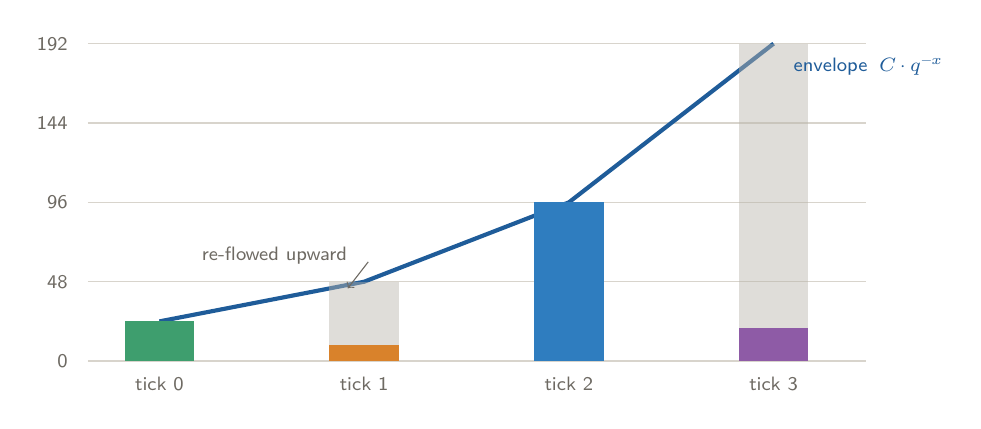
\begin{tikzpicture}[x=2.6cm,y=0.021cm]
  \draw[rulec,line width=0.5pt] (-0.35,0) -- (3.45,0);
  \foreach \v in {0,48,96,144,192}{
    \draw[rulec,line width=0.4pt] (-0.35,\v) -- (3.45,\v);
    \node[soft,font=\scriptsize\sffamily,anchor=east] at (-0.4,\v) {\v};}
  % envelope E(x) = C * q^{-x}, C=24
  \draw[accent,line width=1.5pt] (0,24) -- (1,48) -- (2,96) -- (3,192);
  \foreach \i/\c/\a/\env in {0/cT0/24/24, 1/cT1/10/48, 2/cT2/96/96, 3/cT3/20/192}{
    \fill[\c] (\i-0.17,0) rectangle (\i+0.17,\a);
    \node[soft,font=\scriptsize\sffamily,anchor=north] at (\i,-4) {tick \i};}
  % overflow (what the envelope would have poured into the capped ticks)
  \fill[dead,opacity=0.45] (1-0.17,10) rectangle (1+0.17,48);
  \fill[dead,opacity=0.45] (3-0.17,20) rectangle (3+0.17,192);
  \node[accent,font=\scriptsize\sffamily,anchor=west] at (3.05,178) {envelope $\;C\cdot q^{-x}$};
  \node[soft,font=\scriptsize\sffamily,anchor=west] at (0.16,64) {re-flowed upward};
  \draw[soft,->,line width=0.4pt] (1.02,60) -- (0.92,44);
\end{tikzpicture}
\caption{The same draw, seen as one curve. Every tick that survives sits \emph{exactly} on the
envelope $C\cdot q^{-x}$ — check $96/24 = 4 = q^{-2}$. Every tick that exhausted sits below it,
and the shaded gap above such a bar is precisely the emission that re-flowed to the survivors.}
\end{figure}

That single observation — survivors lie on one geometric curve, and only the exhausted ticks
depart from it — is the whole reason the next section works.

% ==========================================================================
\section{The accumulator: why this is cheap}
\label{sec:acc}

Read naively, every tick's state depends on everything consumed above it, across all history.
That is unaffordable on chain. Factorisability removes the dependence.

Between events the live set, the top $\tau$ and $W$ are constant, so tick $i$ drains at a
constant rate $R\,q^{\tau-i}/W$. Define one global accumulator advancing at
\[
  \mathrm{d}G \;=\; \frac{\mathrm{d}T}{R\,W},
\]
where $T$ is cumulative emission. Then over \emph{any} interval,
\[
  \boxed{\;\text{tokens taken by tick } i \;=\; q^{\,\tau-i}\cdot R\cdot \Delta G\;}
\]

One scalar describes every live tick simultaneously. Reading a tick costs one exponentiation
and no iteration — no per-bidder loop, no history walk, no off-chain indexer. A tick that
nobody touches costs nothing at all.

The waterfall of \S\ref{sec:ex1} is \emph{not} a second algorithm bolted on. It is the same $G$
advancing at piecewise-constant speed, and the speed changes whenever $W$ changes. That buys a
property worth having: the result is \textbf{path-independent}. A single draw of $280$ tokens
produces exactly the outcome of four rounds of $70$.

\subsection{The example, recomputed from one number}

Take the four rounds of \S\ref{sec:ex1} again and track only $G$. When the top of book moves
from $\tau$ to $\tau'$, everything held in ``units of the top'' is rescaled by $q^{\tau-\tau'}$:

\begin{center}
\begin{tabular}{llrr}
\toprule
& segment & $\Delta G$ & $G$ after \\
\midrule
rounds 1--2  & $140$ t at $W=1.75$          & $+1.1429$ & 1.1429 \\
round 3a     & $18.73$ t at $W=1.75$        & $+0.1529$ & 1.2958 \\
             & \emph{tick 2 exhausts; top moves $2\!\to\!1$; rescale} $\times q$ & & 0.6479 \\
round 3b     & $51.27$ t at $W=1.5$         & $+0.4883$ & 1.1362 \\
round 4      & $70$ t at $W=1.5$            & $+0.6667$ & \textbf{1.8028} \\
\bottomrule
\end{tabular}
\end{center}

Tick 2's exhaustion key was predictable in advance:
$100/(70\times1.1025\times1) = 1.2958$ — precisely where $G$ arrived. And now read the two
survivors straight off the final $G$, with $\tau=1$:
\[
  a_0 = R\,q^{1-0}\,G = 70\times0.5\times1.8028 = 63.10,
  \qquad
  a_1 = R\,q^{0}\,G = 70\times1.8028 = 126.20 .
\]

Both match the round-by-round totals in \S\ref{sec:ex1} exactly. Four rounds, one mid-round
exhaustion and one rescale, recovered from a single stored scalar and one exponentiation
each.

\subsection{What that costs in practice}

Three pieces of machinery pay for it:

\begin{itemize}\setlength\itemsep{3pt}
\item \textbf{A rescale on top-of-book changes.} $G$, $W$ and the exhaustion keys are all
      carried in units of the current top; when the top moves they all scale by the same
      $q^{\tau-\tau'}$. Because the factor is common, the \emph{ordering} of the keys is
      untouched — so the rescale is a constant-time operation, never a sweep.
\item \textbf{An ordered structure of exhaustion keys}, for the reason established in
      \S\ref{sec:ex2}. A tick's key changes whenever its budget does, so every bid and every
      withdrawal has to re-file it.
\item \textbf{Aggregate sums for revenue.} Carrying $W_p=\sum p_i q^{\tau-i}$ alongside $W$
      gives revenue and tokens sold per segment without visiting any tick.
\end{itemize}

Worth keeping in proportion: the strict-priority rule of \S\ref{sec:v1} is the $q\to0$ limit of
this scheme. Both run the same number of loop iterations — one per exhausted tick, and each
tick exhausts once. The extra cost is a constant factor inside the loop, not a change in
asymptotics.

% ==========================================================================
\section{The knob}

$q$ interpolates continuously between the two degenerate rules:

\begin{center}
\begin{tabular}{ll}
\toprule
$q \to 0$ & strict price priority — the current mechanism \\
$q = 1$   & equal split across every live tick, price ignored \\
\bottomrule
\end{tabular}
\end{center}

In a dense book the top tick's share is
\[
  \frac{1-q}{1-q^{\,n}} \;\longrightarrow\; 1-q ,
\]
so $q$ sets a soft ceiling on the top of the book: $q=0.75$ caps it near $25\%$ of each round,
$q=0.9$ near $10\%$. The participation window runs roughly $\log_q(\text{dust})$ ticks down —
at $q=0.9$, several hundred levels; at $q=0.5$, about sixty.

Note the qualifier: that ceiling holds only when the book is dense beneath the top. A hard cap
under \emph{any} book shape requires a separate overlay and is not provided by $q$ alone.

The incentive to bid higher stays continuous throughout. Moving up one tick multiplies your
fill rate by $1/q$ in exchange for a price one tick worse — a smooth trade of price against
urgency, rather than a bet on where a threshold will land.

% ==========================================================================
\section{Properties and limits}

\paragraph{No clearing price, twice over.} As in any pay-as-bid design there is no single
price at which everyone transacts. The geometric variant also dissolves the sharp marginal
boundary, so there is not even a ``last filled tick'' to quote. Where a reference price
is needed downstream, the two available ones are the top of book $\tau$ and the realised
average $\mathrm{raised}/\mathrm{sold}$.

\paragraph{Splitting a bid.} A bidder who fragments one budget across $k$ ticks collects $k$
weights instead of one. The friction against this is the minimum bid size times $k$, plus the
genuinely worse fill rate of every level below their best. Whether that friction suffices is
an open calibration question; a concave budget-weight or an explicit cap would close it.
Bidding from several addresses cannot be handled inside the mechanism at all — that needs a
validation hook.

\paragraph{Anchoring.} Dead, by shift-invariance (\S4.1).

\paragraph{Novelty is the risk.} Each component here is proven in production elsewhere:
virtual-time accumulators with a sorted event queue are how fair-queueing network schedulers
and the Linux CFS scheduler work; lazy $O(1)$ reads through a global index are standard in
staking-reward and lending contracts; the capped waterfall with renormalisation is the
water-filling construction from information theory and the classical bankruptcy problem.

The \emph{combination} is what has not been run in production. Classical matching engines
never split volume between price levels; this design does so deliberately. The economics are
therefore unproven in a way the engineering is not, which is why simulation against realistic
books — and specifically against an adversarial whale — should precede deployment rather than
follow it.

\vspace{1.2em}
\noindent{\color{rulec}\rule{\linewidth}{0.6pt}}
\vspace{0.4em}

\noindent{\footnotesize\color{soft}
Every number in \S\ref{sec:ex1} and \S\ref{sec:ex2} was recomputed from scratch rather than
copied from the spec. The model in \mbox{\texttt{index.html}} implements the same rule; open it
with \mbox{\texttt{?selftest}} to check it against both examples.}

\end{document}
